\documentclass[11pt,a4paper]{article}
\usepackage[margin=1in]{geometry}
\usepackage[T1]{fontenc}
\usepackage{lmodern,microtype,amsmath,amssymb,amsthm,booktabs,graphicx,natbib}
\usepackage{enumitem,float,placeins,xurl}
\usepackage[colorlinks=true,linkcolor=black,citecolor=black,urlcolor=blue]{hyperref}
\usepackage[font=small,labelfont=bf]{caption}
\usepackage{setspace}
\setstretch{1.12}
\setlength{\parskip}{3pt}
\setlength{\emergencystretch}{2em}
\newtheorem{proposition}{Proposition}
\newtheorem{corollary}{Corollary}
\newcommand{\R}{\mathbb R}
\newcommand{\pos}[1]{\left[#1\right]_+}
\newcommand{\TotalRoutes}{86557}
\newcommand{\TotalScenarios}{96}
\newcommand{\FirstYear}{2017}
\newcommand{\LastYear}{2024}
\newcommand{\MaxResidual}{1.73e-15}
\newcommand{\MaxGap}{3.59e-11}
\newcommand{\BaseRoutes}{11506}
\newcommand{\BaseValue}{236.13}
\newcommand{\BaseQuantity}{672.29}
\title{Protecting Importers or Protecting Routes?\\[3pt]\large Export Expansion and Reallocation in Food and Fertilizer Trade}
\author{Shivam Gupta\\\normalsize Independent Researcher\\\normalsize\href{mailto:shivam1720406@gmail.com}{shivam1720406@gmail.com}}
\date{14 October 2026}
\begin{document}
\maketitle
\begin{abstract}
Can disrupted imports be restored without reducing the deliveries retained by other importing countries? The answer depends on whether protection attaches to bilateral routes or to importer totals. We develop an inverse trade stress test that computes the export availability growth required under each interpretation and measures the incumbent shipments that must be reassigned. A specialization of classical network-flow theory yields an exact cut characterization for uniform recovery targets and a sharp bound on the value of route flexibility. Applying the framework to six food and fertilizer products in CEPII BACI, 2017--2024, we find substantial heterogeneity. With the 2021 network and complete removal of Ukrainian exports, restoring 95\% of aggregate lost soybean imports requires 14.25\% growth among remaining exporters when surviving routes are protected, but 0.70\% when surviving importer totals are protected. The corresponding wheat thresholds are both approximately 10.79\%. The soybean difference survives persistent-route and fivefold route-expansion screens, while a twofold route ceiling makes both policies infeasible. These are conditional requirements for export availability, not estimates of spare production capacity or causal effects of the war. Historical route entry and country-level recovery constraints delimit their policy interpretation.
\end{abstract}
\noindent\textbf{Keywords:} international trade; supply disruption; export availability; reallocation; food security; network flows.\\
\textbf{JEL codes:} F14, F17, Q17, C61.

\section{Introduction}
A country that loses an important foreign supplier may find that another exporter already produces and sells the same product. That observation leaves two questions unanswered. Does the alternative exporter have enough additional availability? Could it redirect existing deliveries without creating further import losses elsewhere? A bilateral sourcing plan can conceal both constraints. Conversely, protecting every existing bilateral shipment can rule out useful reallocations even when all importing countries could retain the quantities that survived the original shock.

This paper measures the difference between these protection rules. Under \emph{route protection}, each surviving bilateral shipment is a lower bound on subsequent deliveries. Replacement must therefore come entirely from additional export availability. Under \emph{importer protection}, each country's total surviving imports are a lower bound, but the supplying countries can change. A replacement shipment to one importer can then be supported by a chain of adjustments involving other exporters and importers. Every participant retains its surviving import quantity; some bilateral deliveries decline.

The distinction is relevant to international coordination after disruptions to essential goods. National buyers, commodity merchants, and food-security agencies can differ over whether a supply assurance protects an existing seller--buyer relationship or the importer's aggregate access. The World Bank's account of wheat trade after the invasion of Ukraine documents adjustment through alternative suppliers and routes, alongside important regional differences \citep{worldbank}. Such adjustment is not evidence that all lost supply was replaced, or that alternative purchases imposed no costs elsewhere. It does motivate an accounting framework that makes the protection obligation explicit.

Our central object is an \emph{import-preserving restoration frontier}: the minimum common proportional increase in surviving exporters' availability compatible with a declared restoration target, trading support, and permission to reassign incumbent shipments. The approach reverses the usual stress-test question. Instead of interpreting a multiple of historical exports as measured spare capacity, it asks how much additional availability would be required. Historical trade determines the reference scale and observed relationships. Availability growth remains a scenario variable.

We make three contributions. First, we formulate the route-versus-importer comparison while retaining all observed importing economies within each product network. For a uniform recovery target, we specialize the classical max-flow/min-cut condition into a transparent formula indexed by importer coalitions. It shows which group of importers creates a requirement above the global accounting minimum. Second, we quantify coordination through the minimum volume of surviving bilateral shipments that must be withdrawn and replaced. A residual-network interpretation and a cut-based lower bound distinguish additional supply from reassignment effort. Third, we evaluate the framework using six separately analyzed HS17 products and eight annual trade networks, with a fixed 2021 benchmark, alternative support definitions, bilateral route ceilings, and a subsequent-year description.

The empirical result is not a general claim that coordination eliminates scarcity. For wheat and maize in the 2021 Ukraine-removal scenario, the aggregate export loss accounts for almost all the required availability growth. In soybeans, however, a narrow alternative-supplier set for Belarus generates a substantially higher route-protection requirement. Allowing other importers to switch suppliers reduces this bottleneck. Removing both Russia and Ukraine produces a different result: the same narrow access structure can remain restrictive even with reassignment. Expanding the eligible support to relationships observed in 2019--2021 changes that conclusion, showing that market access and shipment reassignment are distinct policy margins.

Our estimates are conditional feasibility calculations. They do not identify harvest responses, contract rights, equilibrium prices, transport capacity, nutrition, or welfare. In particular, the 95\% benchmark refers to aggregate lost tonnage, not 95\% recovery for every affected country. We report the stricter country-level target separately. These qualifications are integral to the economic object being measured: the frontier is a screening tool for the requirements of a protected restoration plan.

\section{Related research and the contribution's boundary}
Research on diversification and resilience already demonstrates that sourcing decisions interact with network rigidities and shock exposure. \citet{ahn} develops a quantitative trade model of diversification and the resilience--efficiency tradeoff. \citet{grossman} studies resilience investment and network formation in vertical supply chains. Our framework does not estimate those equilibrium responses or derive an optimal subsidy. It conditions on a trading support and computes a physical-quantity feasibility requirement.

Shared alternatives are also established. \citet{erokhin} explicitly evaluates joint supplier budgets and competition among national diversification plans. \citet{gupta} develops a linear-programming input--output framework combining trade reallocation and production expansion, with unequal final-demand consequences. We therefore do not claim that shared exporter budgets, endogenous reallocation, or linear programming for trade disruptions are new. Our narrower contribution is to impose a comprehensive surviving-import floor and measure the inverse expansion--reassignment frontier under different meanings of protection. The input--output model of \citet{gupta} represents production linkages that our simpler shipment-accounting model omits.

A substantial food-trade literature studies network fragility, efficiency, and shock propagation. \citet{puma} analyzes evolving systemic vulnerability; \citet{karakoc} examines efficiency and resilience in food-trade networks; \citet{verschuur} evaluates compound shocks in a global crop-trade model. Our focus is the protection constraint and its associated resource requirements, rather than a new claim that food networks transmit shocks.

Trade reconfiguration can also change the meaning of an observed partner. \citet{freund} distinguishes direct sourcing changes from persistent indirect linkages. \citet{gaskin} applies inverse optimal transport to agricultural trade and the Ukraine shock. We do not infer bilateral trade costs or treat gross exports as domestic value added. The mathematical foundation is classical transportation and network-flow theory \citep{ford}. The cut formulas below are specialized accounting identities and their policy interpretation, not a claim to a new max-flow theorem.

\section{Data and research design}
\subsection{Source, products, and coverage}
We use the January 2026 release of CEPII BACI, HS17, covering 2017--2024. BACI reconciles export and mirror-import declarations and adjusts their valuation basis \citep{baci}. Trade values are in thousands of current US dollars and quantities in metric tonnes. We obtain the official ZIP archive through HTTP range requests, validate the CRC32 of every extracted annual member, retain the selected product rows, and record hashes of both the uncompressed members and the retained files. The replication package contains the selected data and acquisition script.

The six products are wheat other than seed (100199), maize other than seed (100590), barley other than seed (100390), soybeans other than seed (120190), crude sunflower-seed or safflower oil (151211), and urea (310210). We analyze each code separately. In particular, the oil category includes safflower oil; its short table label is ``crude seed oil.'' Tonnes are not added across products in any optimization or recovery target. The baskets cover traded staples, an oilseed, edible oil, and a fertilizer input, with different exporter concentration and sourcing structures. They are a purposive selection, not a representative sample of all traded goods.

\begin{table}[htbp]\centering\small
\caption{The 2021 product networks}\label{tab:coverage}
\begin{tabular}{lrrrrrr}
\toprule
HS17 & Product & Exporters & Importers & Routes & Mt & USD bn \\
\midrule
100199 & Wheat & 115 & 193 & 1718 & 189.94 & 53.27 \\
100590 & Maize & 157 & 206 & 2619 & 202.82 & 52.42 \\
100390 & Barley & 109 & 175 & 1293 & 46.70 & 11.67 \\
120190 & Soybeans & 136 & 190 & 1802 & 164.27 & 80.77 \\
151211 & Crude seed oil & 104 & 189 & 1547 & 9.54 & 11.99 \\
310210 & Urea & 132 & 200 & 2527 & 59.01 & 26.00 \\
\bottomrule
\end{tabular}

\begin{minipage}{\textwidth}\footnotesize\textit{Notes:} Positive-quantity, positive-value bilateral flows. Mt denotes million tonnes; values are billions of current US dollars. Counts vary by product. Source: CEPII BACI HS17, release 202601, and the author's calculations.\end{minipage}
\end{table}

Across the eight years, the usable data contain \TotalRoutes{} product--country-pair--year observations. The 2021 benchmark contains \BaseRoutes{} usable routes and USD~\BaseValue{} billion in trade. We remove observations with missing or nonpositive quantities, nonpositive values, or identical exporter and importer codes. The raw 2021 selected extract has 11,618 rows, including 112 with missing quantities; these account for approximately 0.0043\% of its recorded value. It has no duplicate product--pair records or self-flows. The yearly cleaning ledger is included with the code. Quantities are reconciled statistical records, not audited engineering capacities; missing or unreported relationships are not established physical impossibilities.

\subsection{Benchmark, scenarios, and eligible relationships}
The main baseline is 2021, preceding the invasion of Ukraine. We consider complete removal of (i) Ukrainian exports and (ii) both Russian and Ukrainian exports, within each selected product. The latter is labeled the joint-removal scenario. It is a hypothetical loss of exporter availability, not a description of sanctions, Black Sea port traffic, or actual Russian trade in 2022. Import demand in the removed exporting countries remains in the network. Annual exercises for 2017--2024 apply the same hypothetical removals to each year's own network; they are sensitivity comparisons, not repeated observations of the same treatment.

The main support contains every positive observed 2021 surviving-exporter relationship. A three-year union admits additional relationships observed in 2019--2021, while retaining the 2021 quantities and exporter scales. The persistent-material screen permits an increase only on routes with at least USD~100,000 of trade in at least two of those three years. Other existing routes remain in the baseline and may decline under reassignment, but cannot increase. This avoids deleting incumbent imports merely to strengthen the support screen.

We also cap final shipments on each surviving route at two, five, or ten times its 2021 quantity. These are sensitivity restrictions, not estimated route capacities. The nominal-value exercise replaces quantity with recorded value throughout a product network. It checks dependence on the accounting unit; it does not convert nominal values into physical supply. We developed the question and sensitivity comparisons through exploratory analysis. No sampling-based or causal significance claims are attached to the optimization differences.

\section{An import-preserving restoration model}
\subsection{Accounting and protection rules}
Fix one product and year. Let $q_{ji}\geq0$ denote baseline shipments from exporter $j$ to importer $i$. Remove an exporter set $H$. For surviving exporters $j\notin H$, define
\begin{align}
 E_j&=\sum_i q_{ji}, & b_{ji}&=q_{ji},\\
 B_i&=\sum_{j\notin H}q_{ji}, & \ell_i&=\sum_{j\in H}q_{ji}, & D_i&=B_i+\ell_i.
\end{align}
Here $B_i$ is the quantity retained by importer $i$ after the direct removal and $\ell_i$ its direct loss. Let $E=\sum_{j\notin H}E_j=\sum_i B_i$ and $L=\sum_i\ell_i$. Exporter and importer are separate roles: a country can occupy both. The model does not identify its domestic production or net consumption from these roles.

Let $A$ be the eligible surviving-exporter--importer support and $y_{ji}$ post-adjustment shipments. A common increase $\rho\geq0$ limits total availability by
\begin{equation}\sum_i y_{ji}\leq(1+\rho)E_j\quad(j\notin H).\label{eq:availability}\end{equation}
This is a proportional availability envelope referenced to observed exports. It is not a measurement of unused capacity and does not assert that identical percentage expansion is technologically attainable across exporters.

Importer protection requires
\begin{equation}B_i\leq\sum_j y_{ji}\leq D_i\quad\text{for every }i.\label{eq:floor}\end{equation}
No importer can lose any of the quantity it retained after the original shock. A route-release parameter $\delta\in[0,1]$ additionally imposes
\begin{equation}y_{ji}\geq(1-\delta)b_{ji}\quad((j,i)\in A),\qquad y_{ji}=0\quad((j,i)\notin A).\label{eq:release}\end{equation}
At $\delta=0$, every surviving delivery is protected. At $\delta=1$, only importer totals are protected. Intermediate values limit withdrawal from each route separately. The baseline support is always included; additional union-support edges have $b_{ji}=0$.

For an aggregate restoration target $\tau\in[0,1]$, require
\begin{equation}\sum_{ji}y_{ji}\geq E+\tau L.\label{eq:aggregate}\end{equation}
The frontier $\rho^*_{\tau}(\delta)$ minimizes $\rho$ subject to \eqref{eq:availability}--\eqref{eq:aggregate} and nonnegativity. Infeasibility is recorded as $+\infty$, rather than repaired by relaxing the target or opening unobserved routes. The main empirical target is $\tau=0.95$; full restoration uses $\tau=1$.

A distinct, stricter \emph{uniform} target replaces the lower bound in \eqref{eq:floor} with $B_i+\tau\ell_i$ for every importer. We denote its frontier $\rho^u_{\tau}(\delta)$. The distinction matters: an aggregate target can leave a small affected country entirely unrestored while meeting its global tonnage objective. At $\tau=1$, the two targets coincide.

\begin{figure}[htbp]\centering
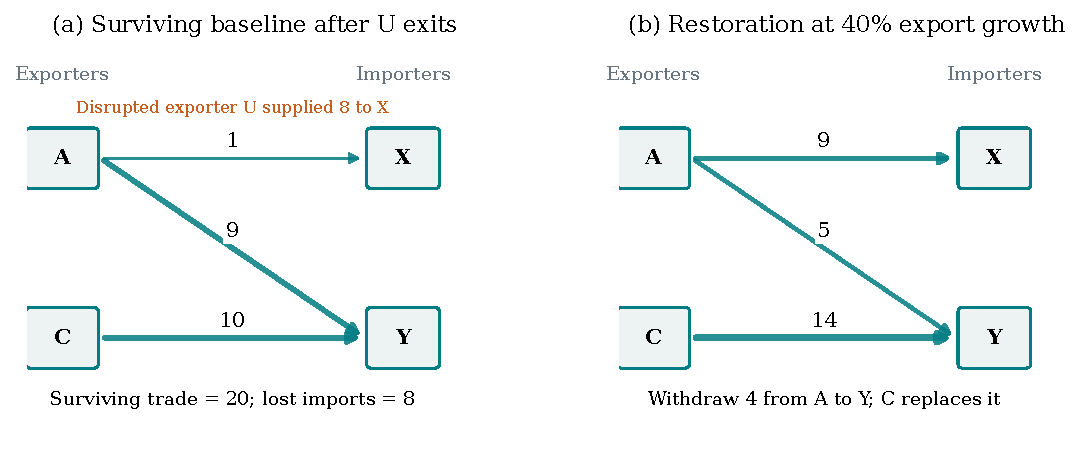
\includegraphics[width=\textwidth]{figures/mechanism.pdf}
\caption{Reassignment can preserve importers while reducing required expansion. After exporter U's eight units disappear, the surviving flows are A--X: 1, A--Y: 9, and C--Y: 10. Route protection requires 80\% expansion because only A supplies X. With reassignment, A supplies X: 9 and Y: 5, while C supplies Y: 14. Both surviving exporters expand by 40\%, X's lost imports are restored, and Y retains all 19 units. Four incumbent units are reassigned. This is a constructed illustration, not an empirical observation.}\label{fig:mechanism}
\end{figure}

\subsection{A cut characterization}
For an importer subset $S$, write $B(S)=\sum_{i\in S}B_i$, $\ell(S)=\sum_{i\in S}\ell_i$, and let $N(S)$ be its eligible surviving suppliers. Define $E(N(S))=\sum_{j\in N(S)}E_j$. In this subsection, eligible routes have no separate upper limits.

\begin{proposition}[Uniform-target frontier]\label{prop:hall}
Assume positive total surviving exports and a support containing every surviving baseline route. Then
\begin{equation}
\rho^u_{\tau}(\delta)=\max\left\{0,\max_{S\subseteq I}\left[\frac{\tau\ell(S)+\delta B(S)}{E(N(S))}-\delta\right]\right\}.\label{eq:hall}
\end{equation}
A positive numerator with zero denominator makes the frontier infinite. A zero-over-zero subset imposes no restriction.
\end{proposition}
\begin{proof}
Subtract the mandatory route floor: $x_{ji}=y_{ji}-(1-\delta)b_{ji}$. Exporter $j$ can supply at most $(\rho+\delta)E_j$ residual units. Importer $i$ needs at least $\tau\ell_i+\delta B_i$. Since the target is no larger than $D_i$, excess deliveries can be deleted, so exact residual-demand equalities suffice. Construct a source--exporter--importer--sink network, with these capacities and demands and unlimited arcs on $A$. By max-flow/min-cut \citep{ford}, all residual demand can be delivered if and only if every importer subset's demand is at most the capacity of its neighboring exporters. Rearranging those inequalities and imposing $\rho\geq0$ gives \eqref{eq:hall}.
\end{proof}

At full restoration, route protection gives $\max_S\ell(S)/E(N(S))$, whereas importer protection gives $\max_S D(S)/E(N(S))-1$, truncated at zero. The whole-importer-set cut implies $\rho\geq\tau L/E$. This global accounting bound also applies to the aggregate target. A larger threshold identifies a distribution or access restriction beyond the global loss of available exports.

\begin{corollary}[Value and limits of route release]\label{cor:lipschitz}
When the uniform-target frontier is finite, it is nonincreasing, convex, and piecewise affine in $\delta$. For $0\leq\delta_1\leq\delta_2\leq1$,
\begin{equation}0\leq\rho^u_{\tau}(\delta_1)-\rho^u_{\tau}(\delta_2)\leq\delta_2-\delta_1.\label{eq:lipschitz}\end{equation}
The bound is sharp.
\end{corollary}
\begin{proof}
Every affine term in \eqref{eq:hall} has slope $B(S)/E(N(S))-1\in[-1,0]$, because surviving baseline deliveries to $S$ are part of its suppliers' total exports. Taking their maximum together with zero proves the properties. For sharpness, consider a disrupted importer whose eligible surviving supplier sells all its baseline exports to another importer, while the disrupted importer was served only by the removed exporter. Admit the new supplier relationship in $A$. The disrupted importer's cut has $B(S)=0$ and slope $-1$. If it remains binding over an interval, equality holds there. A sufficiently well-supplied alternative exporter for the other importer makes the construction feasible.
\end{proof}

The corollary concerns the uniform-target model with unrestricted eligible-route upper bounds. The empirical aggregate-target and capped-route frontiers are solved directly as linear programs. We do not infer their exact shape from this corollary.

\subsection{How much coordination is required?}
Define the volume withdrawn from surviving bilateral deliveries as
\begin{equation}W(y)=\sum_{(j,i)\in A}\pos{b_{ji}-y_{ji}}.\label{eq:withdrawal}\end{equation}
An aggregate reassignment budget $\kappa$ adds $W(y)\leq\kappa E$. This differs from the route-specific release parameter: $\delta$ limits each route, whereas $\kappa$ limits total withdrawn tonnage. Introduce $z_{ji}\geq b_{ji}-y_{ji}$ and $z_{ji}\geq0$ to formulate either the budget or the minimum-withdrawal problem as a linear program.

Let $R_F(\rho)$ be the maximum aggregate lost imports restored under route protection at growth $\rho$, subject to the importer upper bounds. It is an ordinary replacement max flow with exporter capacities $\rho E_j$ and importer capacities $\ell_i$.
\begin{proposition}[A lower bound on reassignment]\label{prop:withdrawal}
With unrestricted eligible-route upper bounds, any importer-protected plan restoring at least $\tau L$ aggregate units satisfies
\begin{equation}W(y)\geq\pos{\tau L-R_F(\rho)}.\label{eq:withdrawbound}\end{equation}
The bound can be attained, but need not be attained when restoration requires a chain of incumbent adjustments.
\end{proposition}
\begin{proof}
For any importer subset $S$, the plan must restore at least $\tau L-\ell(I\setminus S)$ units within $S$. Its suppliers can direct at most $\rho E(N(S))$ extra units there without withdrawing incumbent deliveries to other importers. Thus $W(y)\geq\tau L-\ell(I\setminus S)-\rho E(N(S))$. The max-flow/min-cut formula gives $L-R_F(\rho)=\max_S\{\ell(S)-\rho E(N(S))\}$. Maximizing the preceding inequality over $S$ and imposing nonnegativity proves the result. The example in Figure~\ref{fig:mechanism} attains it.
\end{proof}

A complementary interpretation uses the residual graph of the surviving baseline. Forward exporter-to-importer arcs permit additional deliveries; reverse importer-to-exporter arcs withdraw incumbent deliveries and carry a unit cost. Source arcs represent additional exporter availability, and terminal arcs represent restoration of lost imports. Minimum-cost flow then counts the incumbent withdrawals needed along an adjustment chain. These reverse arcs describe replacement of supply relationships, not physical shipment of goods backward from an importer. Appendix~\ref{app:proofs} gives the construction and explains why a shipment ledger is a feasibility witness rather than an implementable contract.

\section{Results}
\subsection{Scarcity and access differ across products}
Table~\ref{tab:main} reports the minimum growth needed to restore 95\% of aggregate direct losses. Each calculation protects every importer's surviving total, and ``routes'' additionally protects each surviving bilateral shipment. The aggregate columns show $0.95L/E$, the arithmetic lower bound before access or route restrictions.

\begin{table}[htbp]\centering\small
\caption{Required export availability growth in 2021 (percent)}\label{tab:main}
\begin{tabular}{lrrrrrr}
\toprule
 & \multicolumn{3}{c}{Ukraine removal} & \multicolumn{3}{c}{Russia and Ukraine removal}\\
\cmidrule(lr){2-4}\cmidrule(lr){5-7}
Product & Aggregate & Routes & Importers & Aggregate & Routes & Importers \\
\midrule
Wheat & 10.79 & 10.79 & 10.79 & 32.26 & 32.27 & 32.26 \\
Maize & 13.02 & 13.02 & 13.02 & 14.89 & 14.90 & 14.89 \\
Barley & 12.27 & 14.21 & 12.27 & 23.99 & 25.06 & 23.99 \\
Soybeans & 0.70 & 14.25 & 0.70 & 1.25 & 144.70 & 44.70 \\
Crude seed oil & 90.71 & 92.25 & 90.71 & 220.70 & 227.69 & 224.62 \\
Urea & 2.02 & 2.13 & 2.02 & 14.71 & 14.72 & 14.71 \\
\bottomrule
\end{tabular}

\begin{minipage}{\textwidth}\footnotesize\textit{Notes:} Target: 95\% of aggregate lost quantity within each product. ``Aggregate'' is the accounting lower bound, ``routes'' protects surviving bilateral quantities, and ``importers'' permits reassignment while preserving surviving importer totals. Values are required increases relative to all remaining exporters' baseline shipments. They are not measured spare capacity.\end{minipage}
\end{table}

In the Ukraine-removal scenario, wheat and maize lie essentially on the global accounting bound under both protection rules. Reassignment therefore adds little to their optimistic quantity feasibility. Crude seed oil exhibits a different constraint: Ukraine accounts for approximately 48.85\% of baseline quantity, and even importer protection requires approximately 90.71\% growth among the remaining exporters. That is a requirement too large to interpret casually as available short-run slack. Coordination cannot create the missing global quantity.

Soybeans show the largest protection wedge in the Ukraine-removal benchmark. The required growth falls from 14.25\% under route protection to 0.70\% under importer protection, a 13.56 percentage-point difference. Barley falls from 14.21\% to 12.27\%; urea from 2.13\% to 2.02\%. Thus the question is not whether reassignment is always valuable, but which constrained importer sets make it valuable.

\begin{figure}[htbp]\centering
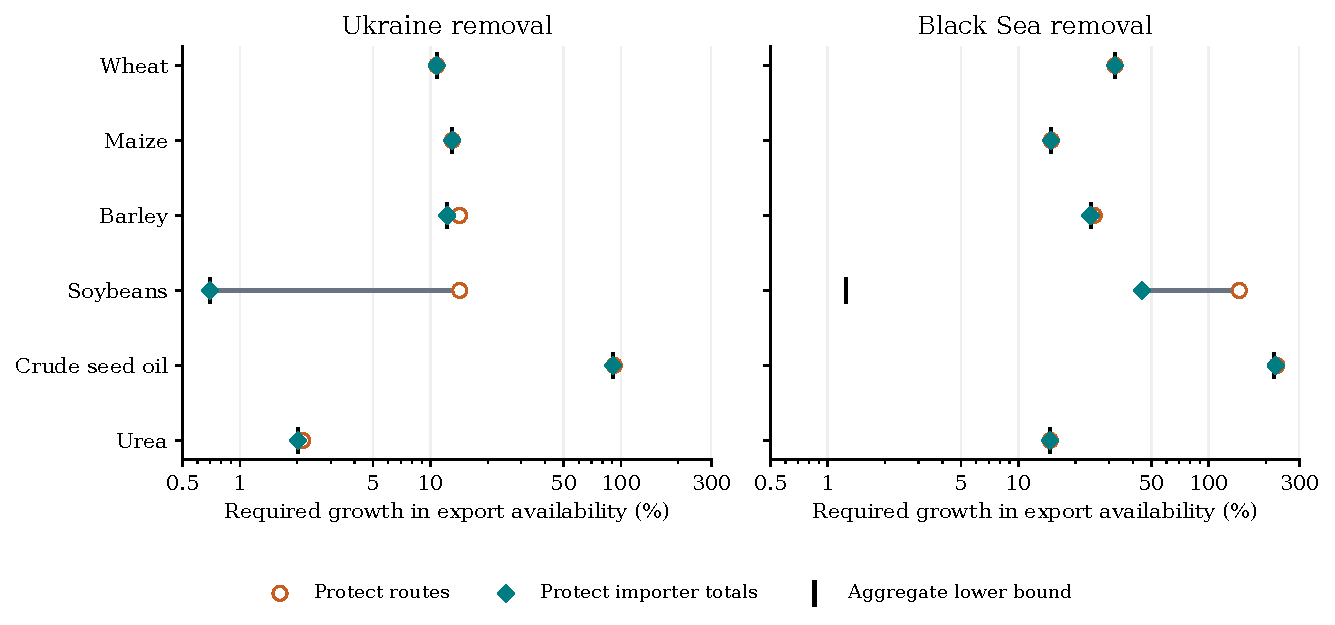
\includegraphics[width=\textwidth]{figures/thresholds.pdf}
\caption{Protection rules and the aggregate availability bound. All points refer to the 2021 network and 95\% aggregate restoration. Horizontal distances use a logarithmic growth axis; overlapping markers indicate nearly identical thresholds. The joint-removal scenario removes Russian and Ukrainian exporter availability, rather than a geographic set of port routes.}\label{fig:thresholds}
\end{figure}

The joint-removal experiment also separates coordination from market access. For soybeans, the route and importer thresholds are 144.70\% and 44.70\%, both far above the 1.25\% global bound. Permitting reassignment helps, but cannot provide a large supplier that is absent from the eligible support. For crude seed oil, the importer-protected threshold exceeds 224\%. These outcomes are signals that the declared restoration package cannot be justified by modest additional availability on the assumed network.

\subsection{The soybean bottleneck and its reassignment requirement}
Belarus's 2021 soybean imports in the usable data are 211,590.749 tonnes from Ukraine, 86,891.207 tonnes from Russia, and 0.005 tonnes from France. Its eligible alternative suppliers therefore have very different scales from the world's dominant soybean exporters. Protecting all incumbent shipments forces replacement through additional availability at those suppliers. Allowing their other buyers to substitute suppliers can free existing shipments for Belarus.

The full-restoration route-protection solution has a cut witness consisting of Belarus. Its requirement is approximately 19.69\%, compared with approximately 0.73\% under importer protection. The 95\% \emph{aggregate} target reduces the former to 14.25\%, in part because the model can leave some direct loss unrestored. Requiring 95\% restoration \emph{at every importer} instead gives 18.71\% under route protection and 0.70\% under importer protection. The conclusion therefore survives the stricter country-level target for this product, while the distinction changes the magnitude of the route-protection requirement.

At the importer-protected aggregate threshold, the minimum-withdrawal program requires approximately 157 thousand tonnes of surviving bilateral soybean shipments to be reassigned, or 0.0964\% of all surviving soybean trade. These calculations use a growth allowance $10^{-7}$ above the computed threshold to avoid solving a secondary program at a numerically knife-edge bound. Under the fivefold route ceiling, the corresponding requirement is approximately 178 thousand tonnes. The archived ledgers show which bilateral quantities decline and which replace them; they do not establish that the quality, timing, or contractual terms of those exchanges are acceptable.

\begin{figure}[htbp]\centering
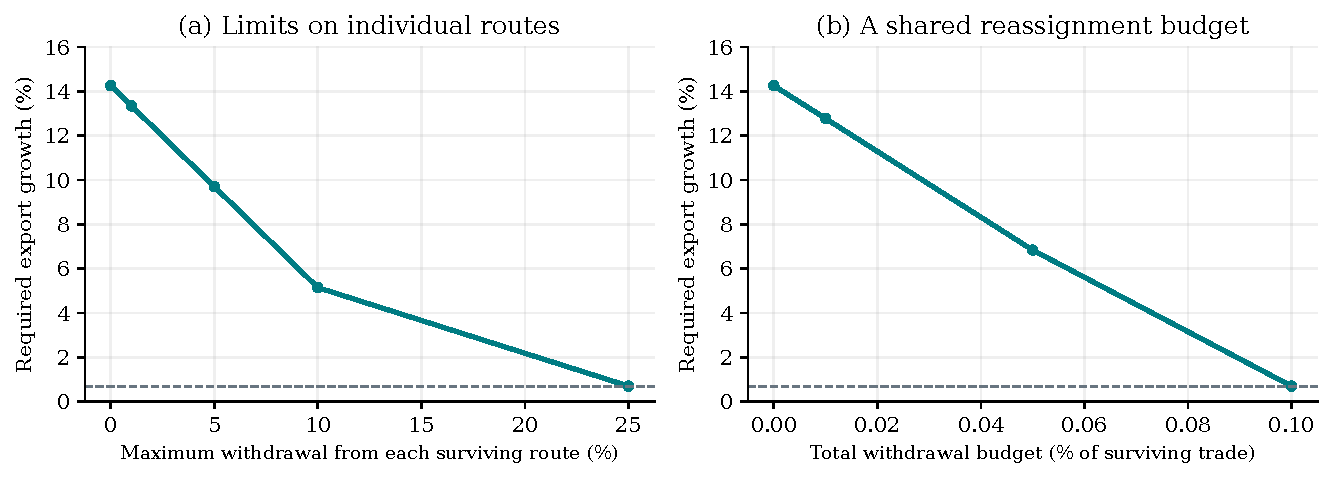
\includegraphics[width=\textwidth]{figures/coordination.pdf}
\caption{The soybean expansion--reassignment tradeoff, 2021 Ukraine removal. Panel (a) limits the fraction withdrawn from each surviving route. Panel (b) limits aggregate withdrawn tonnage relative to surviving world soybean trade. Both target 95\% aggregate restoration. Points are evaluated linear programs, joined for readability. The dashed line marks the unrestricted importer-protected threshold.}\label{fig:coordination}
\end{figure}

Figure~\ref{fig:coordination} distinguishes diffuse flexibility from a small shared budget. A 10\% withdrawal allowance on each route reduces the required growth to approximately 5.14\%. A total withdrawal budget of 0.05\% of surviving trade yields approximately 6.83\%; 0.10\% reaches the aggregate bound. These are quantity tradeoffs rather than monetary valuations of coordination. They leave open whether the reassigned deliveries require compensation, additional transport, or contractual consent.

\subsection{Robustness to trading support and route expansion}
Table~\ref{tab:robust} reports every soybean support and unit specification. The persistent-material screen still produces thresholds of 16.58\% for route protection and approximately 0.70\% for importer protection after Ukraine removal. The result therefore does not require allowing the tiny France--Belarus route to expand. A fivefold ceiling also preserves the difference, at 16.43\% versus 0.70\%. A twofold ceiling makes both policies infeasible. This failure is important: aggregate availability and the ability to scale particular bilateral deliveries are separate requirements.

\begin{table}[htbp]\centering\scriptsize
\caption{Soybean sensitivity: required growth for 95\% aggregate restoration (percent)}\label{tab:robust}
\begin{tabular}{lrrrr}
\toprule
Specification & Ukraine: routes & Ukraine: importers & Both: routes & Both: importers \\
\midrule
2021 support & 14.25 & 0.70 & 144.70 & 44.70 \\
2019--2021 union & 13.17 & 0.70 & 92.37 & 1.25 \\
Persistent material routes & 16.58 & 0.70 & $\infty$ & $\infty$ \\
Route ceiling: twice baseline & $\infty$ & $\infty$ & $\infty$ & $\infty$ \\
Route ceiling: five times baseline & 16.43 & 0.70 & $\infty$ & $\infty$ \\
Route ceiling: ten times baseline & 16.31 & 0.70 & $\infty$ & $\infty$ \\
Nominal value units & 16.76 & 0.79 & 133.05 & 33.05 \\
\bottomrule
\end{tabular}

\begin{minipage}{\textwidth}\footnotesize\textit{Notes:} ``Both'' removes Russia and Ukraine. Persistent material routes have at least USD~100,000 in at least two of 2019--2021; other surviving baseline routes cannot increase. Route ceilings apply to final quantity on every surviving 2021 route. Infinity means the target is infeasible at every exporter expansion factor under those route restrictions. The value-unit exercise is nominal accounting, not a physical capacity estimate.\end{minipage}
\end{table}

For the joint removal, admitting relationships observed during 2019--2021 reduces the importer-protected threshold from 44.70\% to 1.25\%, while the route-protected threshold remains 92.37\%. In contrast, the persistent-material screen makes restoration infeasible. This variation is not an uncertainty interval around a single estimated structural parameter. It measures how the result depends on an explicit definition of eligible trade relationships. The correct operational next step is to verify access and delivery constraints for the relevant suppliers, rather than treating either support as definitive.

Table~\ref{tab:years} in the appendix reports the soybean Ukraine-removal exercise for every available baseline year, including the years in which the difference is small. The protection wedge ranges from 7.76 to 36.14 percentage points in 2017--2021, falls to approximately 0.75 points in 2022, and is below 0.01 points in 2023--2024. This disappearance limits extrapolation from the benchmark to current sourcing networks. The table is a transparent check on dependence on the 2021 snapshot. These later networks already incorporate adaptation and other contemporaneous changes; differences across years do not identify an effect of the war.

\subsection{The aggregate target can leave countries behind}
A 95\% global tonnage target should not be interpreted as broad country-level restoration. In the 2021 barley network, Egypt has no surviving alternative on the observed support after Ukrainian exports are removed. Its loss is approximately 0.387\% of total direct barley losses. A global target can omit that loss and remain feasible, but any positive uniform restoration target is infeasible on this support. This is an accounting statement about observed relationships, not evidence that Egypt cannot obtain barley from another country.

Other full or uniform-target infeasibilities arise from tiny recorded links or quantities. Removing both Russia and Ukraine leaves an isolated affected importer in the soybean data, even though its lost tonnage is negligible globally. A missing alternative for any positive loss prevents complete restoration under a frozen support. We retain these infeasibilities rather than deleting inconvenient markets, and report the aggregate and uniform targets separately in Table~\ref{tab:uniform}.

\subsection{What the following year's trade does and does not validate}
The hypothetical removals deliberately differ from realized 2022 quantities. Ukrainian maize and soybean exports in the usable data increase relative to 2021, while wheat, barley, oil, and urea decline. Figure~\ref{fig:historical} reports these changes and the quantity shares carried by routes absent from the baseline. New or reactivated relationships account for 0.38\% of 2022 soybean quantity, but 8.15\% of urea quantity. Using the three-year union reduces those shares to 0.26\% and 5.33\%, respectively. A static positive-flow support is therefore empirically incomplete, with product-dependent consequences.

\begin{figure}[htbp]\centering
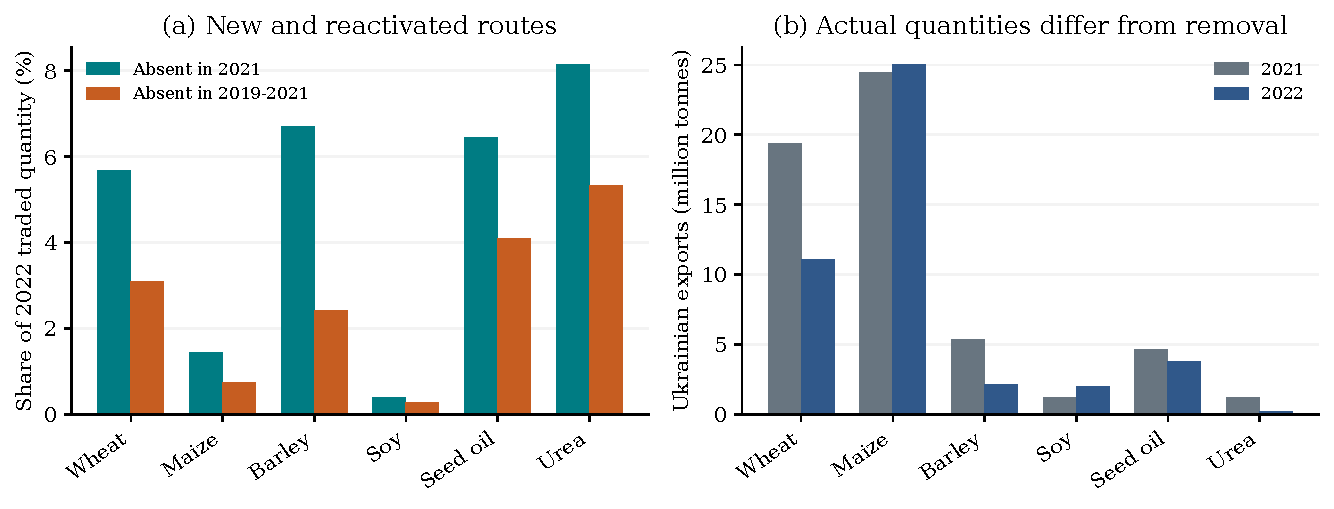
\includegraphics[width=\textwidth]{figures/historical.pdf}
\caption{Observed 2022 quantities delimit the stress test. Panel (a) counts a route as absent if the exporter--importer pair has no usable positive flow in the indicated baseline period within that product. Its denominator is all usable 2022 trade in that product. Panel (b) contrasts actual Ukrainian exports with 2021; complete exporter removal is not an estimate of these changes.}\label{fig:historical}
\end{figure}

These descriptions do not validate a causal counterfactual. Changes in prices, harvests, demand, stocks, classification, re-exports, and logistics can all alter the records. Nor does a new recorded supplier necessarily indicate a new source of domestic production. The role of the subsequent-year exercise is narrower: it rejects treating an observed annual support, or complete exporter removal, as an exhaustive account of actual adjustment.

\section{Policy and commercial interpretation}
The frontier separates three planning margins. The global accounting lower bound measures the additional traded quantity required even on a sufficiently flexible network. A higher importer-protected threshold points to access or allocation restrictions beyond this quantity loss. A difference between route and importer protection measures the value, within the model, of replacing incumbent supply relationships without creating additional importer losses. Bilateral route ceilings can make either plan infeasible even when aggregate exporter growth is unrestricted.

These distinctions change the information needed for policy. A near-binding global constraint calls for evidence on additional export availability, inventories, domestic absorption, and transport. A localized importer cut calls for qualification of alternative suppliers and bilateral access. A substantial reassignment wedge calls for examining which incumbent deliveries could be replaced, who must consent, and whether compensation is feasible. The model identifies quantity requirements for these discussions; it does not rank their welfare benefits.

A practical implementation could support commodity procurement consortia, public food-security planners, or trade-risk teams. The released software accepts a product-level shipment ledger, removes declared suppliers, computes growth and reassignment requirements, and exports a feasible allocation for inspection. Commercial deployment would require private evidence on grade compatibility, plant or port throughput, delivery dates, credit, contracts, and legal access. The existence of a relevant planning problem does not establish customer willingness to pay, a total addressable market, or patentability. The empirical frontier supplies a testable analytical component for such a product, rather than a business valuation.

\section{Limitations}
First, observed exports are reference quantities, not spare capacity. Many capacity configurations can rationalize the same baseline shipments. No optimization of that matrix alone identifies which configuration is real. The frontier is consequently a conditional requirement, and an optimistic one when other unmodeled constraints bind.

Second, a country-product code is not a perfectly homogeneous deliverable. Grain grades, oil composition, fertilizer concentration, shipping seasons, and certification can prevent substitution. The route-cap and support screens expose some dependence on those assumptions but cannot replace product-level verification. Annual data also conceal short-lived shortages and timing mismatches.

Third, the model describes gross international shipments. Re-exports and entrep\^ot trade can make exporter availability depend on imports. We protect importer quantities but do not impose a domestic material-balance or production-function system. The results cannot be interpreted as domestic output responses, food-consumption protection, or an input--output multiplier. Prices, income, transport costs, inventories, preferences, and endogenous export restrictions are outside the model.

Fourth, the aggregate target does not impose equal recovery shares. Uniform targets can be infeasible because an affected importer lacks any observed alternative, including for very small quantities. Neither target measures nutrition or distribution within countries. Normative priority weights would require a separate justification.

Finally, the contribution is a particular measurement and protection comparison using established optimization methods. The literature search identifies close predecessors and narrows the novelty claim; it cannot establish that an equivalent unindexed formulation does not exist. The analysis contains no randomized policy variation, causal elasticity estimate, or evidence that the computed reallocations could be implemented at the required cost.

\section{Conclusion}
Protecting every surviving shipment and protecting every importer's surviving access impose different restoration requirements. The difference is small when a global quantity loss binds, and can be large when an affected importer has a narrow set of alternative suppliers whose incumbent customers can switch elsewhere. The 2021 soybean exercise illustrates the latter case; wheat and maize provide useful contrasts. Route ceilings, alternative support definitions, and country-level targets materially qualify the result. Reporting an export expansion--reassignment frontier makes these requirements explicit and provides a reproducible basis for deciding which availability, access, and contracting evidence a credible restoration plan still needs.

\section*{Data, code, and preparation statement}
The replication archive contains the selected CEPII BACI data, provenance hashes, linear-programming implementation, synthetic tests, empirical outputs, shipment ledgers, and figure and manuscript sources. BACI data remain under the Etalab Open Licence 2.0, with CEPII attribution. Code is provided under the MIT licence. The repository is \url{https://github.com/shi1720/import-restoration-frontiers}.

OpenAI Codex assisted with literature discovery, formulation development, programming, computational checks, and manuscript drafting. The archived numerical results were generated by the supplied scripts. No model-generated image is used as empirical evidence.

\bibliographystyle{plainnat}
\bibliography{references}
\clearpage
\appendix
\section{Additional derivations and implementation}\label{app:proofs}
\subsection{Residual-network construction}
Start from the feasible surviving baseline $b$. For each eligible route $(j,i)$, create a forward arc from exporter role $j$ to importer role $i$ with sufficient capacity for an increase, and a reverse arc from importer role $i$ to exporter role $j$ with capacity $b_{ji}$ and unit cost. Each exporter receives a source arc of capacity $\rho E_j$. Each importer has a terminal arc of capacity $\ell_i$. All other arcs have zero cost. An augmenting path may increase one delivery, withdraw another to the same importer, and then redirect the released supplier's output. Intermediate importer roles have zero net change, so surviving imports are preserved. Terminal flows restore lost imports.

A feasible post-adjustment plan induces signed route changes relative to $b$. Decompose these changes into source--terminal paths and cycles. Cycles restore no additional imports; deleting cycles cannot increase the withdrawal cost. Opposite movements along the same route can also be cancelled. After cancellation, the total reverse-arc flow equals $W(y)$. Thus a minimum-cost flow attaining $\tau L$ restoration minimizes incumbent withdrawal. With finite route ceilings $c_{ji}\geq b_{ji}$, the forward residual capacity becomes $c_{ji}-b_{ji}$; an unsupported route has zero forward capacity. The implementation solves the equivalent linear program, using explicit withdrawal variables, rather than relying on a particular path decomposition.

A path decomposition need not be unique. Even the minimum-withdrawal ledger can have multiple solutions. The printed shipment plan is one feasible witness returned by the solver. It should not be interpreted as a unique prediction, a negotiated allocation, or an equilibrium.

\subsection{Feasibility, certificates, and numerical checks}
For the uniform target without route ceilings, the transformed source capacities are $(\rho+\delta)E_j$ and terminal demands are $\tau\ell_i+\delta B_i$. The cut inequalities in Proposition~\ref{prop:hall} are sufficient as well as necessary; no assumption of independent exporter shocks is used. The formula requires a common expansion multiplier and complete removal of the declared exporter set. It does not describe an arbitrary supplier-specific growth vector without replacing the numerator condition by the corresponding weighted capacity inequalities.

The code uses \texttt{scipy.optimize.linprog} with the HiGHS backend \citep{scipy}. Quantities are scaled so total baseline flow is approximately $10^4$ optimization units, with a minimum scale of one. Primal and dual feasibility tolerances are $10^{-9}$. Reported errors are recomputed from unscaled flows and divided by baseline product trade. We check importer floors and ceilings, target delivery, exporter envelopes, and mandatory route floors. We also compare primal and dual objective values, accounting for bound multipliers. In the archived annual panel, the largest normalized primal residual is \MaxResidual{} and the largest absolute primal--dual objective gap is \MaxGap{}.

For finite full-restoration benchmark solutions, positive importer dual multipliers identify a candidate binding subset. We explicitly reconstruct its eligible exporter neighborhood and evaluate the cut ratio. The maximum gap between those cut bounds and the corresponding LP thresholds in the benchmark is below $10^{-12}$. Infeasibility results are retained separately; no finite certificate is reported for an infeasible solve.

Synthetic verification includes exhaustive enumeration of all importer subsets on 150 randomly generated five-by-five networks at five release levels. These 750 independently evaluated cut formulas agree with the optimization thresholds or their infeasibility status. Further tests cover the worked example, monotonicity, the one-unit bound on the uniform frontier's reduction, a zero-shock case, aggregate budget endpoints, and the withdrawal lower bound on 40 additional random networks. These tests validate implementation against the declared model, not the realism of its economic assumptions.

\section{Supplementary empirical results}
\begin{table}[htbp]\centering\small
\caption{Annual coverage of the selected products}\label{tab:annual}
\begin{tabular}{lrrr}
\toprule
Year & Usable routes & USD bn & Mt \\
\midrule
2017 & 9091 & 149.20 & 561.77 \\
2018 & 9876 & 163.86 & 587.87 \\
2019 & 10542 & 161.21 & 602.21 \\
2020 & 10796 & 177.63 & 658.94 \\
2021 & 11506 & 236.13 & 672.29 \\
2022 & 11863 & 288.54 & 643.12 \\
2023 & 11755 & 247.93 & 649.27 \\
2024 & 11128 & 206.39 & 636.52 \\
\bottomrule
\end{tabular}

\begin{minipage}{\textwidth}\footnotesize\textit{Notes:} Route counts are summed across six separate product networks. Monetary and quantity sums summarize coverage only; optimization never treats products as interchangeable. Missing-quantity observations are excluded.\end{minipage}
\end{table}

\begin{table}[htbp]\centering\small
\caption{Soybeans: annual Ukraine-removal sensitivity, 95\% aggregate target}\label{tab:years}
\begin{tabular}{lrrrr}
\toprule
Baseline year & Aggregate (\%) & Routes (\%) & Importers (\%) & Difference (pp) \\
\midrule
2017 & 1.05 & 8.81 & 1.05 & 7.76 \\
2018 & 1.10 & 24.29 & 1.10 & 23.19 \\
2019 & 1.56 & 37.70 & 1.56 & 36.14 \\
2020 & 1.06 & 17.70 & 1.06 & 16.64 \\
2021 & 0.70 & 14.25 & 0.70 & 13.56 \\
2022 & 1.23 & 1.98 & 1.23 & 0.75 \\
2023 & 1.90 & 1.91 & 1.90 & 0.00 \\
2024 & 1.95 & 1.95 & 1.95 & 0.00 \\
\bottomrule
\end{tabular}

\begin{minipage}{\textwidth}\footnotesize\textit{Notes:} Each row uses that year's own positive-flow support and export quantities. The difference is the route-protection threshold minus the importer-protection threshold, in percentage points. These are hypothetical stress tests on different snapshots, not estimated annual treatment effects.\end{minipage}
\end{table}

\begin{table}[htbp]\centering\small
\caption{Requiring 95\% restoration at every affected importer (percent growth)}\label{tab:uniform}
\begin{tabular}{lrrrr}
\toprule
Product & Ukraine: routes & Ukraine: importers & Both: routes & Both: importers \\
\midrule
Wheat & 10.79 & 10.79 & 32.27 & 32.26 \\
Maize & 13.02 & 13.02 & 14.90 & 14.89 \\
Barley & $\infty$ & $\infty$ & $\infty$ & $\infty$ \\
Soybeans & 18.71 & 0.70 & $\infty$ & $\infty$ \\
Crude seed oil & $\infty$ & $\infty$ & $\infty$ & $\infty$ \\
Urea & 2.13 & 2.02 & 14.72 & 14.71 \\
\bottomrule
\end{tabular}

\begin{minipage}{\textwidth}\footnotesize\textit{Notes:} Uniform target $\sum_j y_{ji}\geq B_i+0.95\ell_i$ for every importer. This differs from Table~\ref{tab:main}'s aggregate target. ``Both'' removes Russia and Ukraine. Infinity reflects infeasibility under the observed support, including isolated importers with small positive losses.\end{minipage}
\end{table}

\begin{table}[htbp]\centering\small
\caption{Minimum incumbent withdrawals near the importer-protected threshold}\label{tab:withdrawals}
\begin{tabular}{lrrr}
\toprule
Product & Growth (\%) & Withdrawals (kt) & Surviving trade (\%) \\
\midrule
Wheat & 10.790 & 5.14 & 0.0030 \\
Maize & 13.021 & 5.06 & 0.0028 \\
Barley & 12.266 & 577.93 & 1.3972 \\
Soybeans & 0.696 & 157.23 & 0.0964 \\
Crude seed oil & 90.711 & 73.90 & 1.5139 \\
Urea & 2.018 & 62.60 & 0.1083 \\
\bottomrule
\end{tabular}

\begin{minipage}{\textwidth}\footnotesize\textit{Notes:} Ukraine removal; 95\% aggregate restoration; unrestricted eligible-route ceilings. Secondary minimization uses the computed threshold plus $10^{-7}$. Withdrawals are decreases in surviving bilateral shipments that are offset by alternative deliveries to preserve each importer's floor. They are not additional import losses. kt denotes thousand tonnes.\end{minipage}
\end{table}

\begin{table}[htbp]\centering\small
\caption{Observed subsequent-year quantities and support changes}\label{tab:observed}
\begin{tabular}{lrrrr}
\toprule
Product & 2021 UA Mt & 2022 UA Mt & New route (\%) & Absent 3yr (\%) \\
\midrule
Wheat & 19.372 & 11.064 & 5.68 & 3.09 \\
Maize & 24.449 & 25.042 & 1.44 & 0.73 \\
Barley & 5.341 & 2.145 & 6.70 & 2.41 \\
Soybeans & 1.195 & 1.991 & 0.38 & 0.26 \\
Crude seed oil & 4.661 & 3.806 & 6.44 & 4.09 \\
Urea & 1.227 & 0.168 & 8.15 & 5.33 \\
\bottomrule
\end{tabular}

\begin{minipage}{\textwidth}\footnotesize\textit{Notes:} UA denotes Ukraine. ``New route'' is the share of 2022 product quantity on pairs absent in 2021. ``Absent 3yr'' uses absence throughout 2019--2021. New country-pair records can reflect new sourcing, reactivation, or statistical recording changes.\end{minipage}
\end{table}
\FloatBarrier
\section{Replication map}
\begin{enumerate}[leftmargin=*,itemsep=3pt]
\item \path{src/fetch_baci.py} retrieves the official archive members, verifies ZIP checksums, and filters the six product codes. \path{data/source_manifest.json} records source size, ETag, uncompressed-member hashes, and selected-data hashes.
\item \path{src/model.py} implements the expansion, recovery, and withdrawal programs. \path{src/test_model.py} supplies independent cut-enumeration and structural checks.
\item \path{src/analyze.py} constructs the annual baseline and scenario panel. \path{src/diagnostics.py} evaluates uniform targets and full-restoration cut certificates.
\item \path{src/robustness.py} computes the support, route-cap, accounting-unit, and reassignment-budget comparisons and the subsequent-year descriptions. \path{src/case_study.py} produces the soybean ledgers and constrained-ledger comparison.
\item \path{src/figures.py} and \path{src/tables.py} regenerate the figures, numerical macros, and tables from the archived results. \path{paper/manuscript.tex} and \path{paper/references.bib} compile the manuscript. The README provides commands and dependency versions.
\end{enumerate}
\end{document}
